\section{Beyond the Standard Model}
Many beyond the SM (BSM) theories have been proposed to address the issues discussed in Section~\ref{sm_status}. Theories such as large extra dimensions address the unnatural Higgs boson mass by allowing gravity to spread across more than three spatial dimensions, which lowers $M_P$ and therefore the size of the Higgs boson mass corrections\fxnote{probably cite ADD}. Other theories, such as supersymmetry, posit new symmetries that protect the Higgs boson mass from large corrections. 

\subsection{Supersymmetry}
Supersymmetry (SUSY) introduces a new symmetry in which every SM particle fits into a larger multiplet with an inherent symmetry between bosons and fermions. In its simplest form, SUSY predicts one new boson for every SM fermion, one new fermion for every SM boson, and one new Higgs doublet. The increase in particle multiplicity necessitates a new naming convention: the spin-0 superpartners of the SM fermions are called sfermions (e.g. sleptons or squarks) while the spin-$\frac{1}{2}$ superpartners to the SM bosons add "ino" to the end of their SM counterpart (e.g. Higgsino or wino).

When calculating contributions to the Higgs boson mass from loop diagrams, one finds that fermion loops differ in sign from boson loops, which means that in SUSY every bosonic correction to the Higgs mass is cancelled by a fermionic correction and vice versa. If SUSY were an exact symmetry of nature, the cancellation would be perfect, and the observed Higgs boson mass would match the bare Higgs boson mass exactly. Figure~\ref{higgs_top_stop_corrections} shows a sample leading-order cancellation.

\begin{figure}[hbtp]
\centering
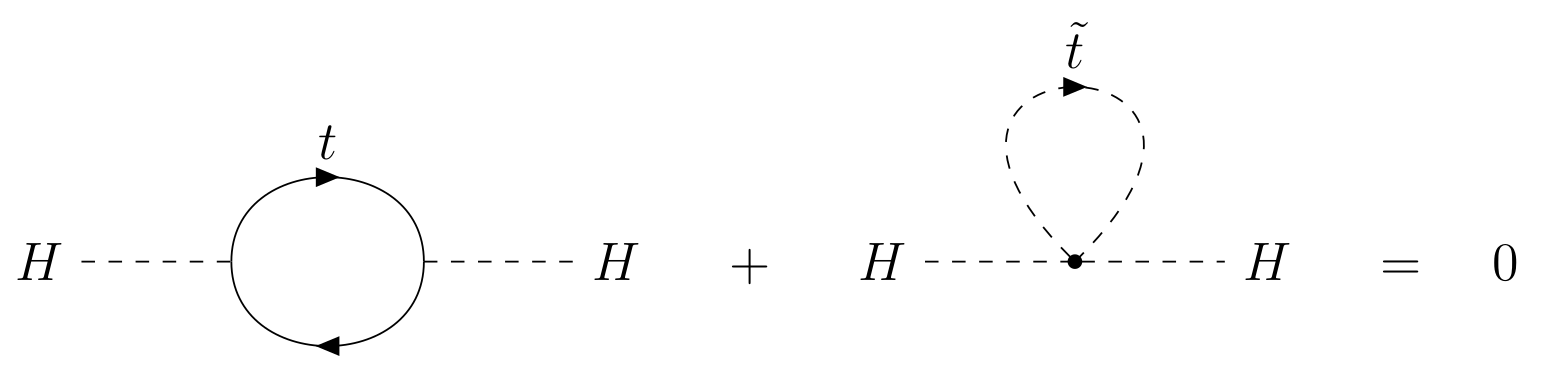
\includegraphics[scale=0.2]{figures/intro/higgs_top_stop_corrections.png}
\caption{Corrections to the Higgs boson mass from the top quark (left) and top squark (right) cancel in exact SUSY. The top quark and top squark contributions are enhanced by the large top--Higgs coupling.}
\label{higgs_top_stop_corrections}
\end{figure}

Exact SUSY also requires that SUSY particles have the same mass as their SM counterparts, so the uniformly null results in collider searches imply that if SUSY exists, it must be a broken symmetry. In broken SUSY, the diagrams in Fig.~\ref{higgs_top_stop_corrections} no longer exactly cancel. Instead, the resulting correction is proportional to the mass of the top squark\fxnote{cite something, probably Craig ([7] in candidacy)}, which means that broken SUSY can still resolve the naturalness problem if the SUSY particles that correct the Higgs boson mass are relatively light.

\fxnote{transition to llps by talking about susy experimental status}
\fxnote{mention gauge coupling, dark matter coupling, etc?}

\subsection{Long-lived particles}
In the context of collider physics, long-lived particles (LLPs) are particles whose lifetimes are such that they decay a measurable distance from the collision point. This category includes everything from particles that decay less than \SI{1}{\mm} away from the collision to particles that propagate through the entire detector. \fxnote{add transition/context sentence after finishing susy section}

SM particles are long lived for many reasons. First, symmetries such as charge and baryon number conservation ensure that particles such as electrons and protons are absolutely stable. Second, small coupling constants and highly virtual intermediate states decrease the decay rate of particles such as muons, whose \SI{2.2}{\us} lifetime is the product of a weak decay through a virtual $W$ boson (the $W$ boson mass is about \num{760} times that of the muon). Finally, limited decay phase space increases the lifetime of particles such as the neutron, whose decay into a proton, an electron, and an electron neutrino is slowed by the near mass degeneracy of the neutron and the proton. The mass difference between the neutron and its decay products is less than \SI{1}{\MeV}. The muon and neutron decays are diagrammed in Fig.~\ref{neutron_muon_decays}.

\begin{figure}
\centering
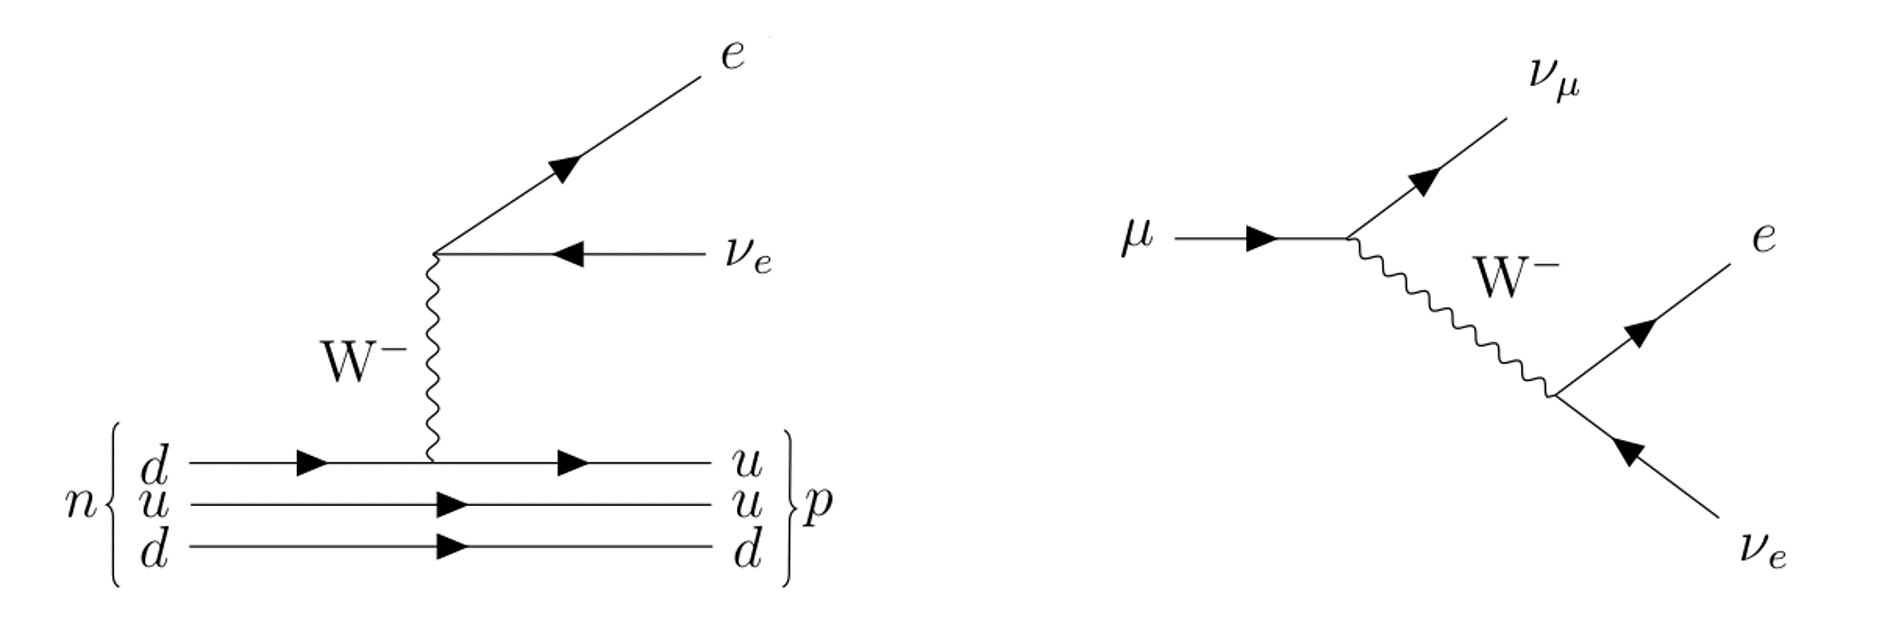
\includegraphics[width=0.9\textwidth]{figures/intro/neutron_muon_decays.pdf}
\caption{Long-lived decays of the neutron (left) and muon (right).}
\label{neutron_muon_decays}
\end{figure}

In BSM physics, the same fundamental mechanisms have the potential to produce new long-lived particles. Many SUSY scenarios, for example, introduce a symmetry known as R parity that prevents proton decay\fxnote{cite something, probably martin}. In models with exact R-parity conservation, SM particles are assigned R-parity \num{+1} and SUSY particles are assigned R-parity \num{-1}. Conserving the product of R-parity at each vertex has two phenomenological consequences: SUSY particles must be produced in pairs, and the lightest SUSY particle (LSP) must be absolutely stable. A neutral, weakly interacting LSP would therefore pass through detectors such as the CMS detector described in Section~\ref{cms} without interacting. The resulting momentum imbalance is a standard signature in SUSY searches \fxnote{cite somebody}.

On the other hand, SUSY models with weakly coupled R-parity violating (RPV) terms produce long-lived but not perfectly stable LSPs \fxnote{cite displaced susy or liu and tweedie}. A similar situation arises in gauge-mediated SUSY breaking models where the gravitino\fxnote{I never defined the graviton} is the LSP. The strength of the coupling between the next-to-LSP (NSLP) and the gravitino is inversely proportional to the energy scale at which SUSY is broken. A high SUSY breaking scale therefore suppresses the NLSP decay rate, making it long lived \fxnote{cite 11 from candidacy}.

LLPs also arise from particular SUSY mass spectra. Models in the Split SUSY paradigm, for example, propose that the spin-0 SUSY particles are significantly more massive than the spin-$\frac{1}{2}$ SUSY particles. In these models, the gluino becomes long lived when its decay to two quarks and a neutral $spin-\frac{1}{2}$ SUSY particle is suppressed by a highly virtual intermediate squark \fxnote{cite "Split supersymmetry at colliders"}. Other SUSY models produce long-lived particles by limiting decay phase space. Some anomaly-mediated SUSY breaking models, for example, predict that the NLSP and LSP are nearly degenerate in mass. Just like the neutron decaying into a proton, the lack of available phase space suppresses the decay and produces a long-lived NLSP \fxnote{\cite{out_of_this_world_susy}}.

In summary, LLPs are a general feature of the SM, and it is reasonable to assume that the same mechanisms that produce SM LLPs will also manifest in BSM physics. The following subsection gives an overview of the phenomenology of the SUSY model most relevant to the analysis presented in Chapter~\ref{displaced_leptons}, while the experimental details of this model and LLP searches at the LHC will be saved until after presenting the LHC and CMS experiment in Chapter~\ref{lhc_and_cms}.

\subsection{Displaced supersymmetry}

% people have been looking for susy for a while
% collider constraints on particle masses are particularly worrying because susy with high-mass sparticles no longer solves the hierarchy problem
% we should therefore look for ways that low-mass sparticle susy could be missed at colliders
% most models assume r-parity to avoid proton decay
% most searches are therefore focused on ptmiss
% possible to introduce rpv without contradicting proton lifetime bounds by allowing terms that violate lepton number but not baryon number
% specifically, bilinear rpv with small couplings is consistent with proton lifetime bounds, works with gauge unification, and leads to long-lived LSPs that would be missed by most collider searches
% 